\chapter{Parte Práctica}
En esta parte se describirá el trabajo realizado para predecir la temperatura máxima durante la próxima semana y durante los dos siguientes meses dependiendo del experimento. El dataset que se ha utilizado corresponde con la estación meteorológica de Reus, Tarragona.

\section{Ejecución de los ficheros de código}
Para la ejecución de los ficheros de código, basta con abrir dichos ficheros en RStudio y pulsar el botón source o la combinación de teclas Ctrl+Alt+R. Para ver los resultados de la ejecución, se debe mirar la terminal que contiene RStudio y el apartado \textit{Plots} que hay a la derecha del IDE para poder mirar las gráficas.

\section{Predicción diaria}
Para este apartado se pide realizar una predicción de la siguiente semana después del último dato del dataset correspondiente. Lo primero que se va a hacer es cargar el dataset y transformar las variables a sus para que sean enteros, fechas, etc... Si nos fijamos en los datos de la serie, el primer dato que contiene es 7 de mayo de 2013 y el último del 28 de febrero de 2018; por lo que el dataset contiene casi 5 años de datos.

\begin{figure}[H]
	\centering
	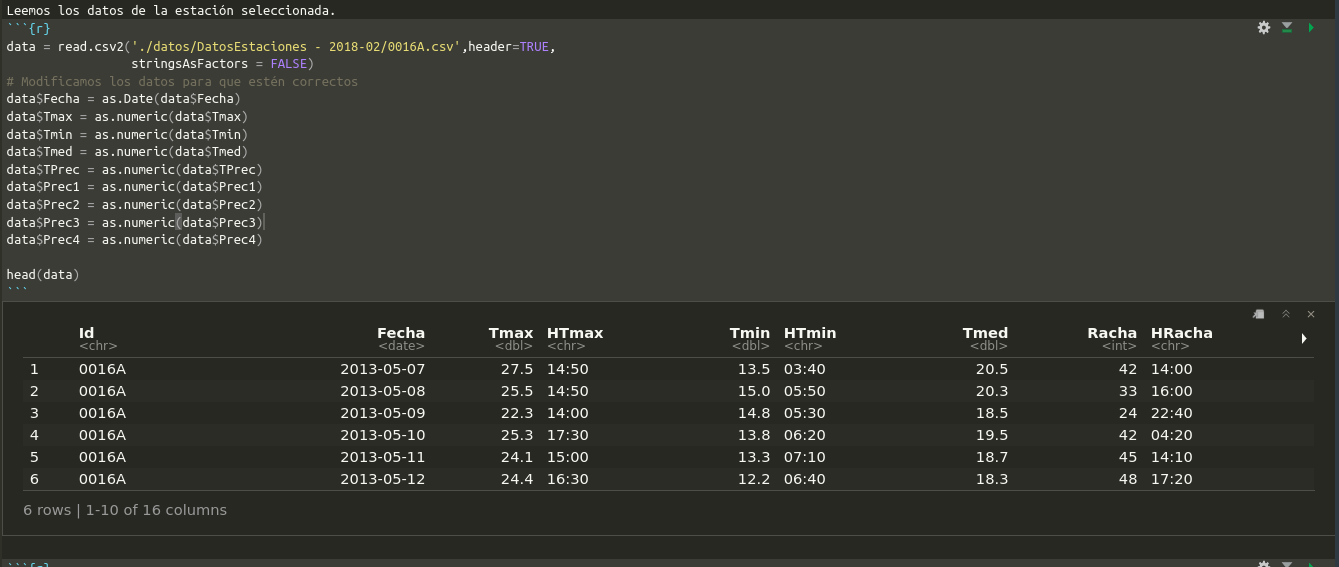
\includegraphics[width=100mm]{imagenes/initial_prep.png}
	\label{fig:1}
	\caption{Transformación de datos del dataset}
\end{figure}

Una vez tenemos los datos cargados y transformados, se debe comprobar si hay datos pérdidos en la columna que vamos a estudiar. Para ello, se selecciona dicha columna junto con la fecha de la medición y se utilizará el método \textit{nic} de la librería \textit{mice} para comprobar si existen datos perdidos; si existen, se imputarán con el método \textit{amelia} de la libería \textit{Amelia}.

\begin{figure}[H]
	\centering
	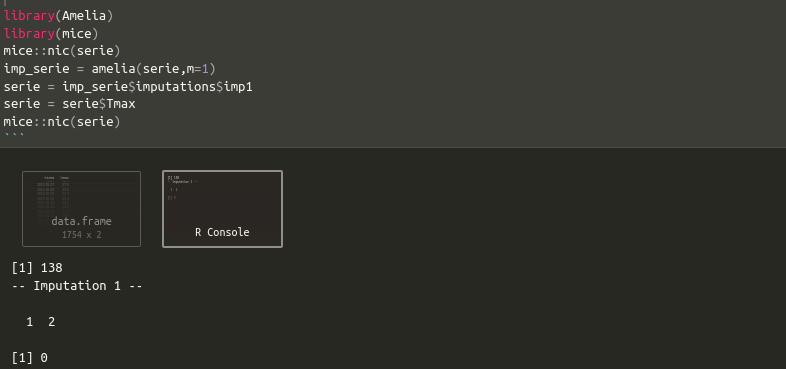
\includegraphics[width=100mm]{imagenes/imputation_diario.png}
	\label{fig:2}
	\caption{Imputación de valores en la serie}
\end{figure}
 
 Ahora, podemos pasar a estudiar la serie al completo, para ello se debe crear un objeto de la clase \textit{ts}; a este objeto se le debe pasar el conjunto de datos de la serie y la frecuencia. Para nuestro caso, la frecuencia se ha estimado como 365, ya que tenemos datos diarios de varios años. Lo siguiente será visualizar la serie temporal y poder ver que forma tiene.
 
 \begin{figure}[H]
 	\centering
 	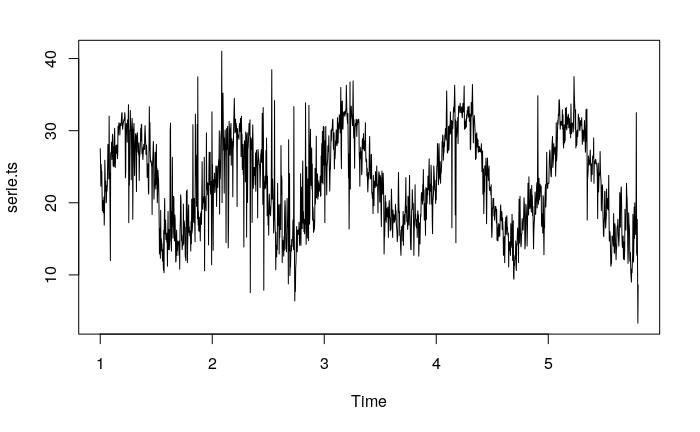
\includegraphics[width=100mm]{imagenes/serie_ts.png}
 	\label{fig:3}
 	\caption{Serie temporal datos diarios}
 \end{figure}

Como se puede ver, la serie tiene mucha variación entre unos días y otros; esto puede hacer que el estudio de modelos de la serie se vea afectado por esta gran variación. Por ello, se va a filtrar la serie haciendo por cada día la media de los quince días de alrededor (la temperatura del día, la de los siete días anteriores  y la de los siete siguientes); de esta forma, se debería conseguir una serie mucho más suave y sin tantos picos. Para ello se utilizará un filtro de convolución sobre la serie. Los resultados son los siguientes.

\begin{figure}[H]
	\centering
	\subfigure[Serie y filtrado]{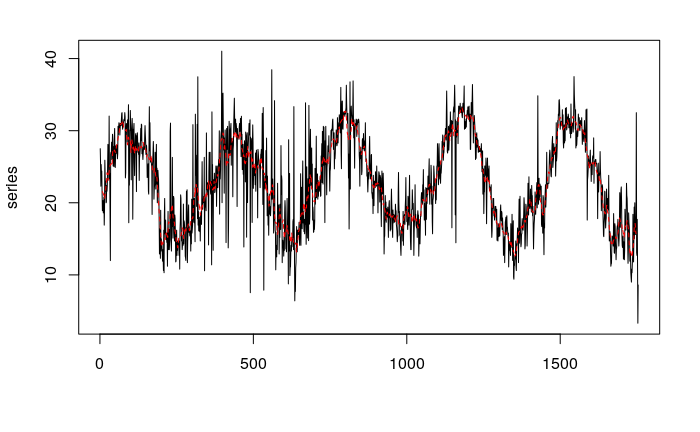
\includegraphics[width=60mm]{imagenes/serie_y_filtro.png}}
	\subfigure[Serie filtrada]{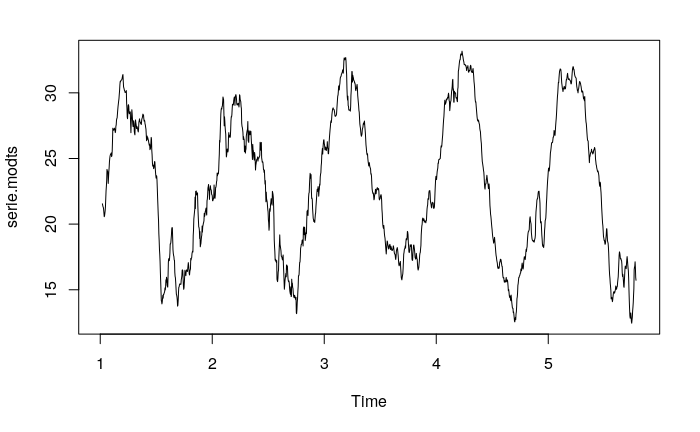
\includegraphics[width=60mm]{imagenes/serie_filtrada.png}}
	\caption{Comparación entre serie filtrada y serie normal}
	\label{fig:4}
\end{figure}

Como se puede ver, esta serie tiene muchos menos picos que la serie normal y será mucho más fácil de analizar. Al haber hecho el filtro sobre la serie, se han perdido algunos valores al principio y al final de la serie, por ello, cuando se vaya a hacer la predicción de la primera semana de marzo, se deberá también predecir estos datos perdidos.

Lo siguiente que se va hacer es realizar un estudio sobre las componentes de la serie, para ello se va a utilizar una descomposición de la serie en sus diferentes componentes y se analizará que tipo de componentes están presentes en la serie y se eliminarán para convertir la serie en estacionaria. La descomposición de la serie es la siguiente.

\begin{figure}[H]
	\centering
	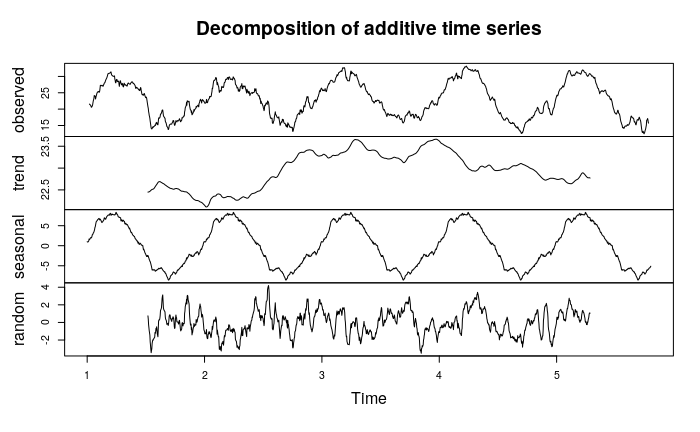
\includegraphics[width=100mm]{imagenes/decomposition.png}
	\caption{Descomposición de la serie}
	\label{fig:5}
\end{figure}

Por lo que se puede ver en la descomposición de la serie, hay una componente estacional clara dentro de los datos; esto es normal en una serie donde se mide la temperatura ya que hay que tener en cuenta las estaciones del año. En la componente de tendencia puede parecer a simple vista que existe una tendencia positiva, pero si nos fijamos en el rango de esta, se puede ver que la serie solamente varia en un grado y medio durante toda la serie; además a partir de la mitad de la serie parece que vuelve a bajar; por lo tanto, se considerará que realmente no tiene una componente de tendencia y no será necesario estudiarla. Lo siguiente que debemos hacer es separar los datos de la serie en un conjunto de validación y en otro de entrenamiento; utilizaremos el conjunto de entrenamiento para modelar la estacionalidad y eliminarla del conjunto de datos y para crear un modelo de predicción, con el conjunto de validación comprobaremos la calidad del modelo de predicción. Para realizar la partición entre train y test, se va a utilizar un conjunto de 4 años para train y el resto de la serie para test.	La separación entre train y test quedaría de la siguiente forma.

\begin{figure}[H]
	\centering
	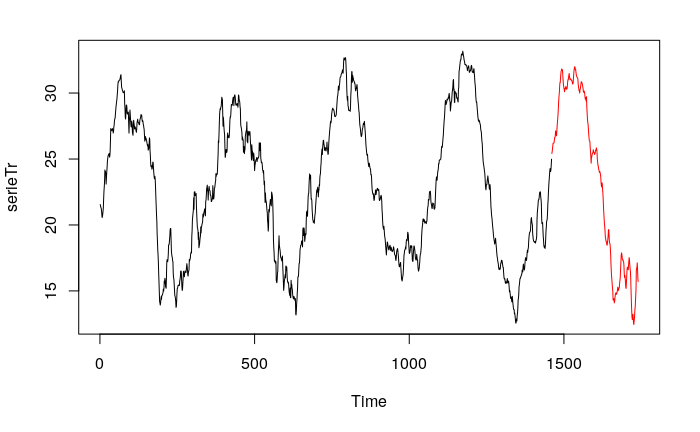
\includegraphics[width=100mm]{imagenes/traintest.png}
	\caption{Separación en train y test}
	\label{fig:6}
\end{figure}

Lo siguiente que vamos a hacer es eliminar la componente estacional de la serie, para ello, obtendremos la componente estacional de la serie mediante la función \textit{decompose}; de los datos que nos devuelve esta función se pueden utilizarán los de un año, para los datos se test se replicará para adaptarse al tamaño de train y para los datos de test se utilizarán solamente los necesarios para el tamaño de test; tras esto se le restará la componente a cada uno de los conjuntos. El resultado es el siguiente.

\begin{figure}[H]
	\centering
	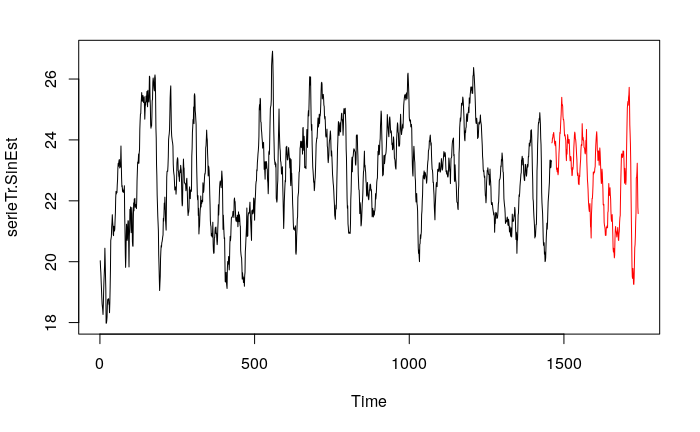
\includegraphics[width=100mm]{imagenes/no_estacional.png}
	\caption{Serie sin estacionalidad}
	\label{fig:7}
\end{figure}

A continuación, tenemos que comprobar si la serie es estacionaria, para ello, se utilizará el test de \textit{Dickey-Fuller} y la gráfica \textit{ACF} de la serie. Si la serie es estacionaria, debe de pasar el test (obtener un p-valor menor que 0.05) y la gráfica debería descender rápida a 0. Los resultados son los siguientes.

\begin{figure}[H]
	\centering
	\subfigure[Resultados test]{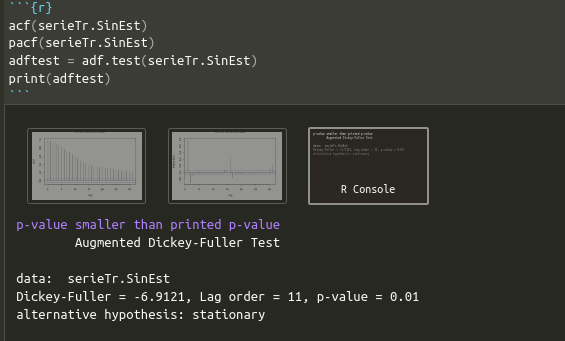
\includegraphics[width=60mm]{imagenes/dickey_fuller_1.png}}
	\subfigure[Gráfica ACF]{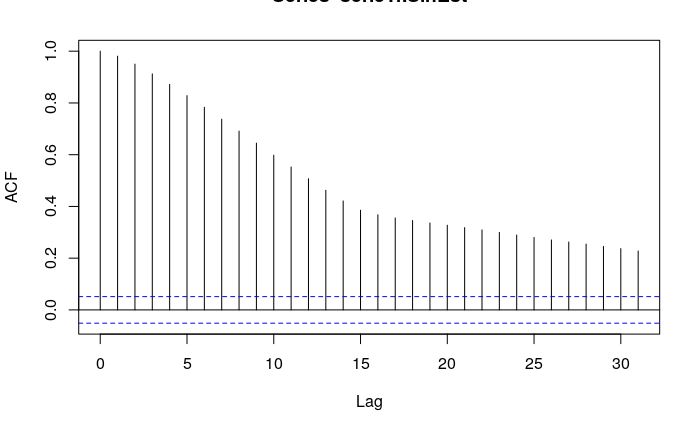
\includegraphics[width=60mm]{imagenes/acf_1.png}}
	\caption{Test Dickey-Fuller y ACF de la serie}
	\label{fig:8}
\end{figure}

Como se puede ver, la serie pasa el test, sin embargo, la gráfica \textit{ACF} no desciende a 0, por lo tanto no es estacionaria. Para conseguir que sea estacionaria, se diferenciará la seria el número de veces que sea necesario hasta que sea estacionaria, para nuestra serie, con una diferenciación ya ha sido suficiente; estos son los resultados.

\begin{figure}[H]
	\centering
	\subfigure[Resultados test]{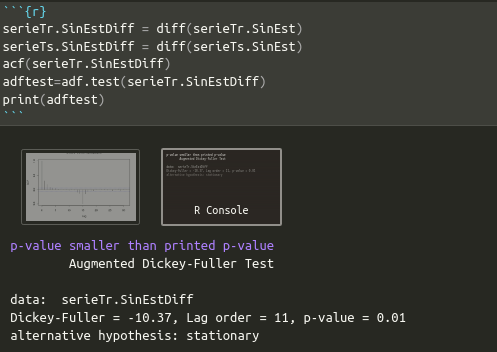
\includegraphics[width=60mm]{imagenes/dickey_fuller_diff.png}}
	\subfigure[Gráfica ACF]{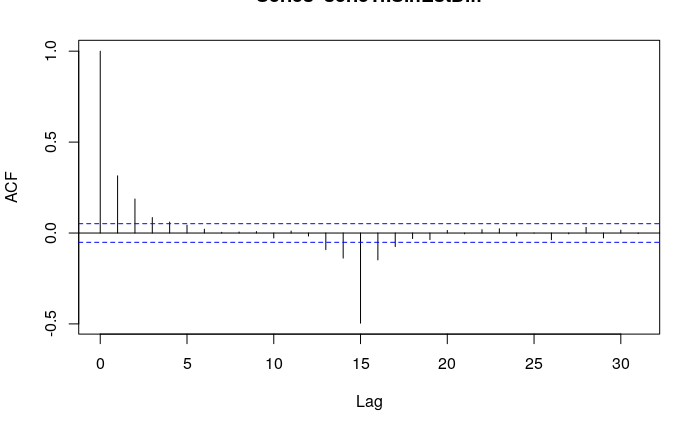
\includegraphics[width=60mm]{imagenes/acf_2.png}}
	\caption{Test Dickey-Fuller y ACF de la serie diferenciada}
	\label{fig:9}
\end{figure}

Ahora, la gráfica sí desciende rápidamente a 0 y pasa el test, por lo que estacionaria. Lo siguiente que vamos a hacer es analizar la gráfica \textit{ACF} y la gráfica \textit{PACF} para saber que tipo de modelo se puede utilizar.

\begin{figure}[H]
	\centering
	\subfigure[Gráfica ACF]{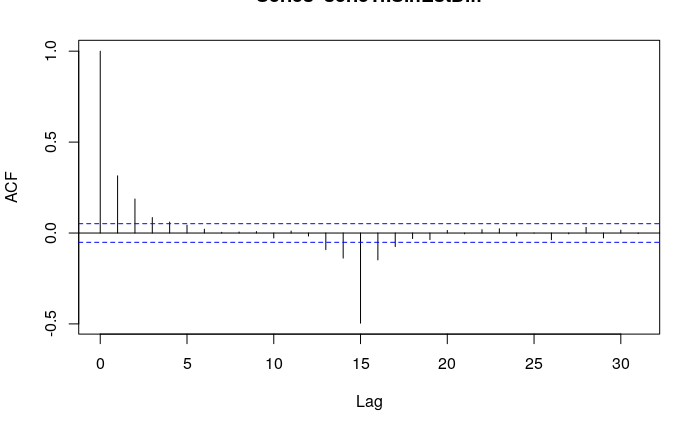
\includegraphics[width=60mm]{imagenes/acf_2.png}}
	\subfigure[Gráfica PACF]{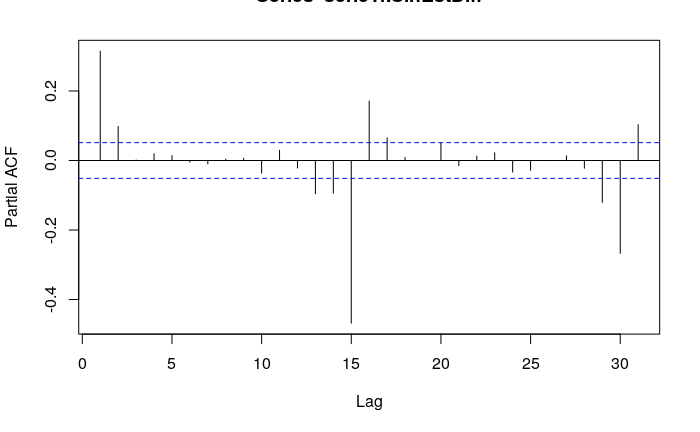
\includegraphics[width=60mm]{imagenes/pacf_2.png}}
	\caption{Gráficas ACF y PACF}
	\label{fig:10}
\end{figure}

Por lo que se puede ver en las gráficas, podría ser un modelo AR(1), un modelo MA(4), o una combinación de ambos. Se crearán los tres modelos y se compararán para ver cuál de ellos es mejor. Para crear los modelos, se utilizará el modelo \textit{ARIMA} indicándole el tipo de modelo; tras esto, se hará una gráfica sobre el ajuste que tiene sobre los datos y la predicción sobre el conjunto de validación. También se utilizarán diferentes test para saber que los modelos obtenidos son correctos.

Para el primer modelo, estos son los resultados obtenidos por los test y el ajuste que tiene con los datos.

\begin{figure}[H]
	\centering
	\subfigure[Ajuste sin estacionalidad]{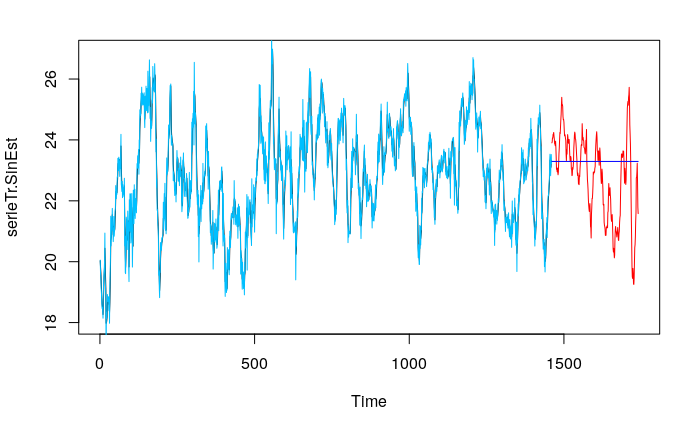
\includegraphics[width=60mm]{imagenes/ajuste_ar1.png}}
	\subfigure[Ajuste con estacionalidad]{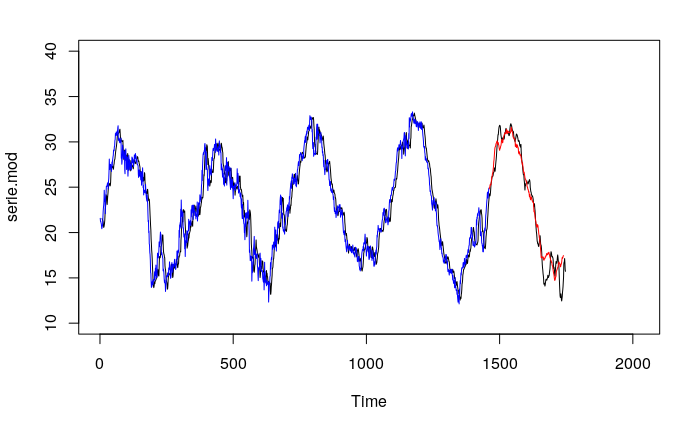
\includegraphics[width=60mm]{imagenes/ajuste_ar1_serie.png}}
	\subfigure[Tests AR1]{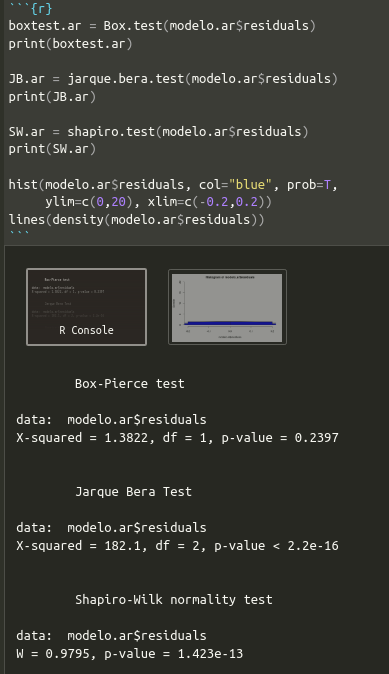
\includegraphics[width=60mm]{imagenes/test_ar1.png}}
	\subfigure[Histograma residuos AR1]{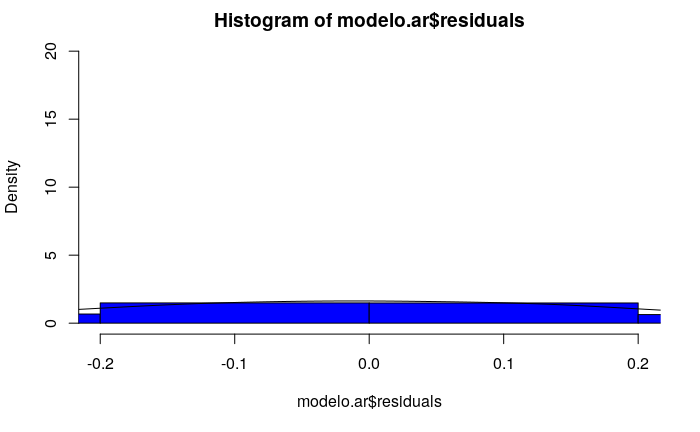
\includegraphics[width=60mm]{imagenes/hist_ar1.png}}
	\caption{Resultados del modelo AR1}
	\label{fig:11}
\end{figure}

Por lo que se puede ver, el modelo generado con AR(1) obtiene un buen ajuste. Los test \textit{Jarque-Bera} y \textit{Shapiro-Wilk} sirven para medir si los residuos del modelo tienen una distribución normal, como el p-valor en ambos es menor que 0.05, pasa el test. El otro test, el test de \textit{Box-Pierce} sirve para saber si los residuos del modelo son aleatorios o no; en este caso es necesario que el p-valor sea  mayor que 0.05, ya que sino estaríamos comprobando que los residuos siguen una distribución no aleatoria, y eso significaría que el modelo está sobreajustándose a los datos, cosa que no queremos. Veamos ahora los resultados obtenidos por los otros dos modelos.

\begin{figure}[H]
	\centering
	\subfigure[Ajuste sin estacionalidad]{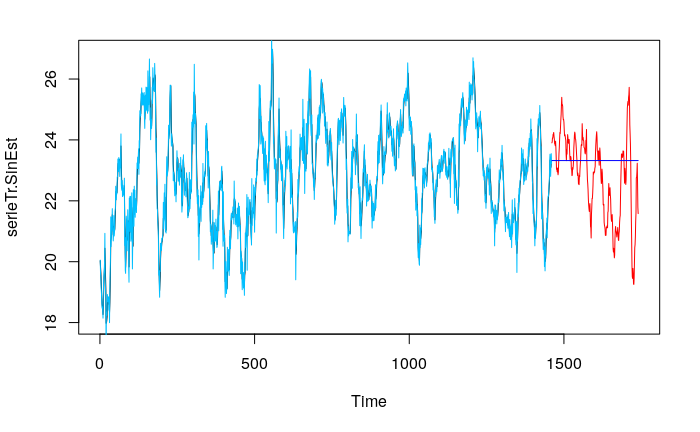
\includegraphics[width=60mm]{imagenes/ajuste_ma4.png}}
	\subfigure[Ajuste con estacionalidad]{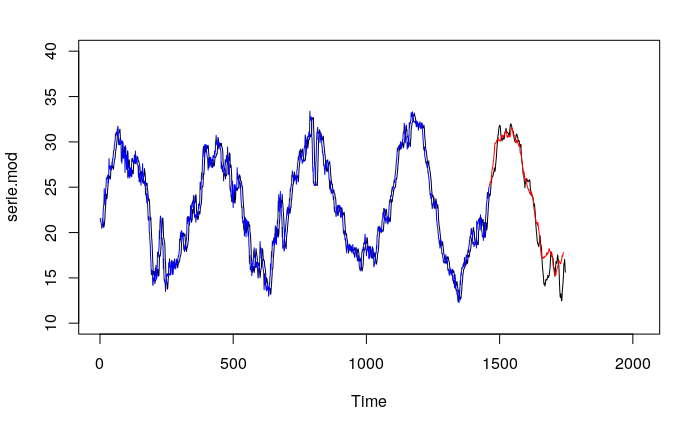
\includegraphics[width=60mm]{imagenes/ajuste_ma4_serie.png}}
	\subfigure[Tests MA4]{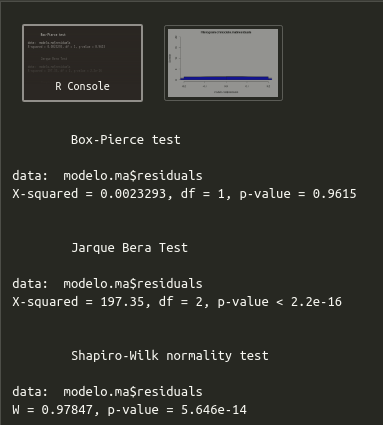
\includegraphics[width=60mm]{imagenes/test_ma4.png}}
	\subfigure[Histograma residuos MA4]{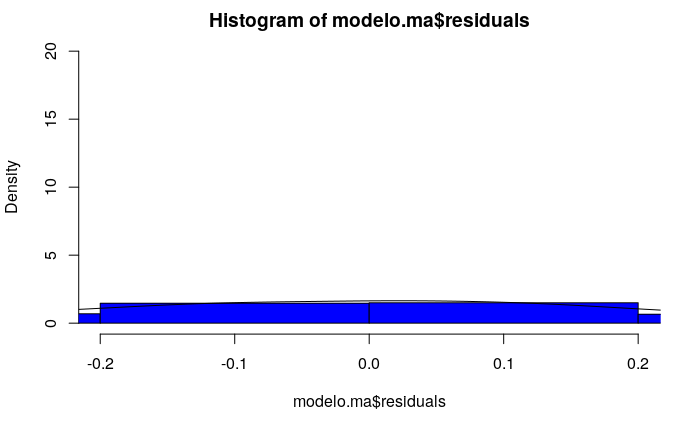
\includegraphics[width=60mm]{imagenes/hist_ma4.png}}
	\caption{Resultados del modelo MA4}
	\label{fig:12}
\end{figure}

\begin{figure}[H]
	\centering
	\subfigure[Ajuste sin estacionalidad]{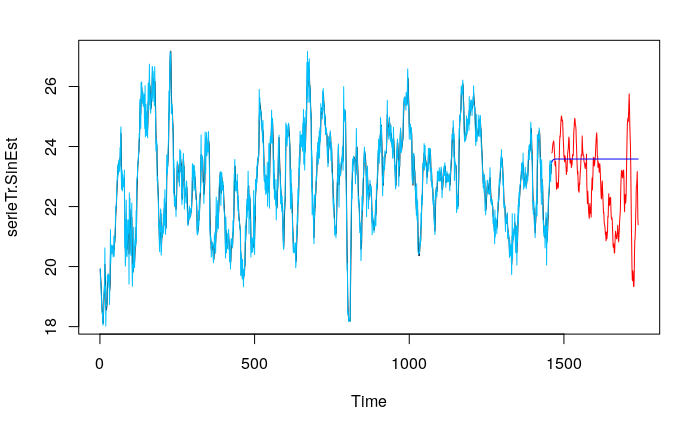
\includegraphics[width=60mm]{imagenes/ajuste_arma.png}}
	\subfigure[Ajuste con estacionalidad]{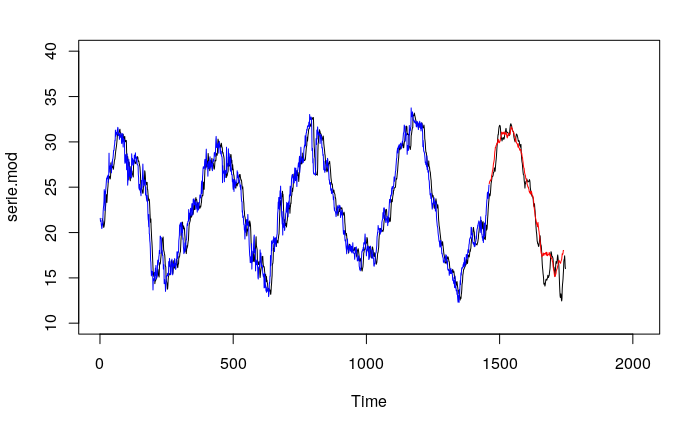
\includegraphics[width=60mm]{imagenes/ajuste_arma_serie.png}}
	\subfigure[Tests ARMA]{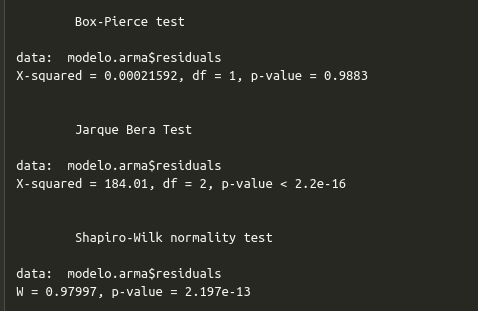
\includegraphics[width=60mm]{imagenes/test_arma.png}}
	\subfigure[Histograma residuos ARMA]{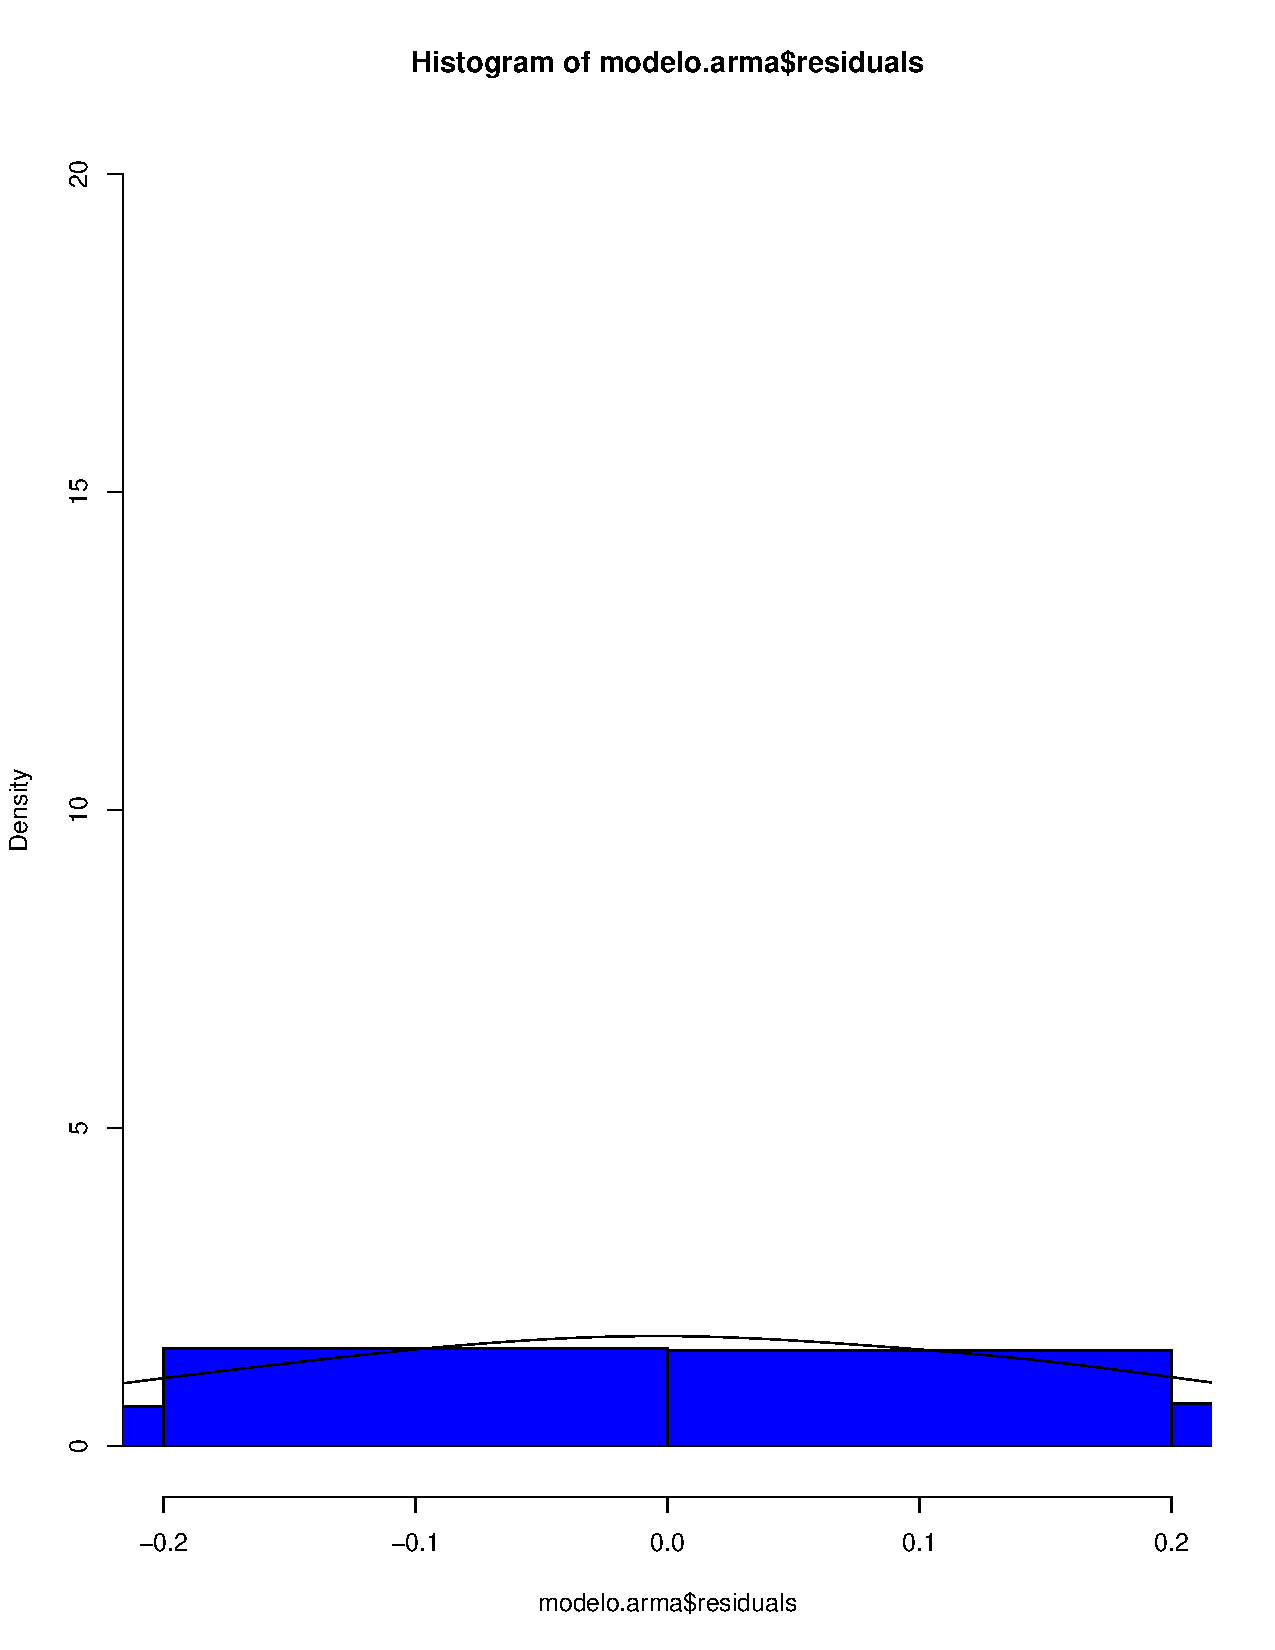
\includegraphics[width=60mm]{imagenes/hist_arma.pdf}}
	\caption{Resultados del modelo ARMA}
	\label{fig:13}
\end{figure}

Como se puede ver, los tres modelos pasan los test y los ajustes son muy parecidos; para elegir a uno de los tres para realizar la predicción, utilizaremos el criterio de AIC y el error producido en test de cada uno de los algoritmos. El error y el resultado del criterio de AIC son los siguientes.

\begin{figure}[H]
	\centering
	\subfigure[Resultados AIC]{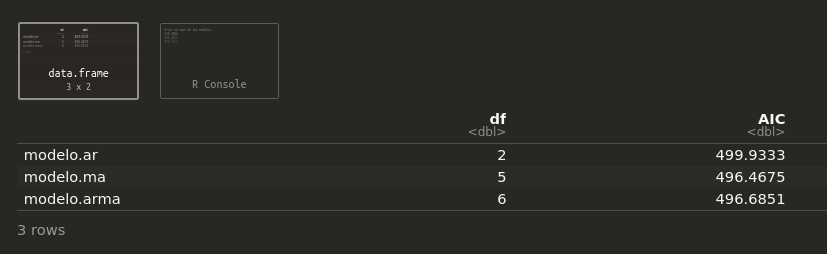
\includegraphics[width=60mm]{imagenes/AIC_diario.png}}
	\subfigure[Error en test]{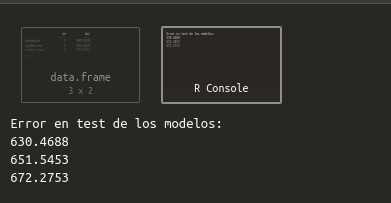
\includegraphics[width=60mm]{imagenes/error_ts.png}}
	\caption{Comparación modelos}
	\label{fig:14}
\end{figure}

Por lo que se vé en la salida del criterio de AIC, los modelos son muy parecidos, el que peores resultados obtiene es el modelo AR(1), aunque este es el más sencillo; los modelos MA(4) y ARMA(1,4) son muy parecidos. Si nos fijamos en el error producido por cada uno de ellos, el que produce el error más pequeño es el modelo AR(1), mientras que los otros modelos obtiene errores mayores conforme se aumenta la complejidad. Por ello, elegiremos el modelo AR(1) para realizar la predicción.

Para realizar la predicción de la siguiente semana, se utilizará la serie entera (con el filtrado). Lo primero será eliminar la estacionalidad, una vez eliminada se construye un modelo AR(1) con una diferenciación. Tras esto se obtiene los valores ajustados y la predicción (recordar, hay que predecir 15 días por el filtrado utilizado). Una vez obtenidos la predicción y el ajuste, se vuelve a añadir la estacionalidad y se muestra la predicción obtenida por el modelo. La predicción es la siguiente.

\begin{figure}[H]
	\centering
	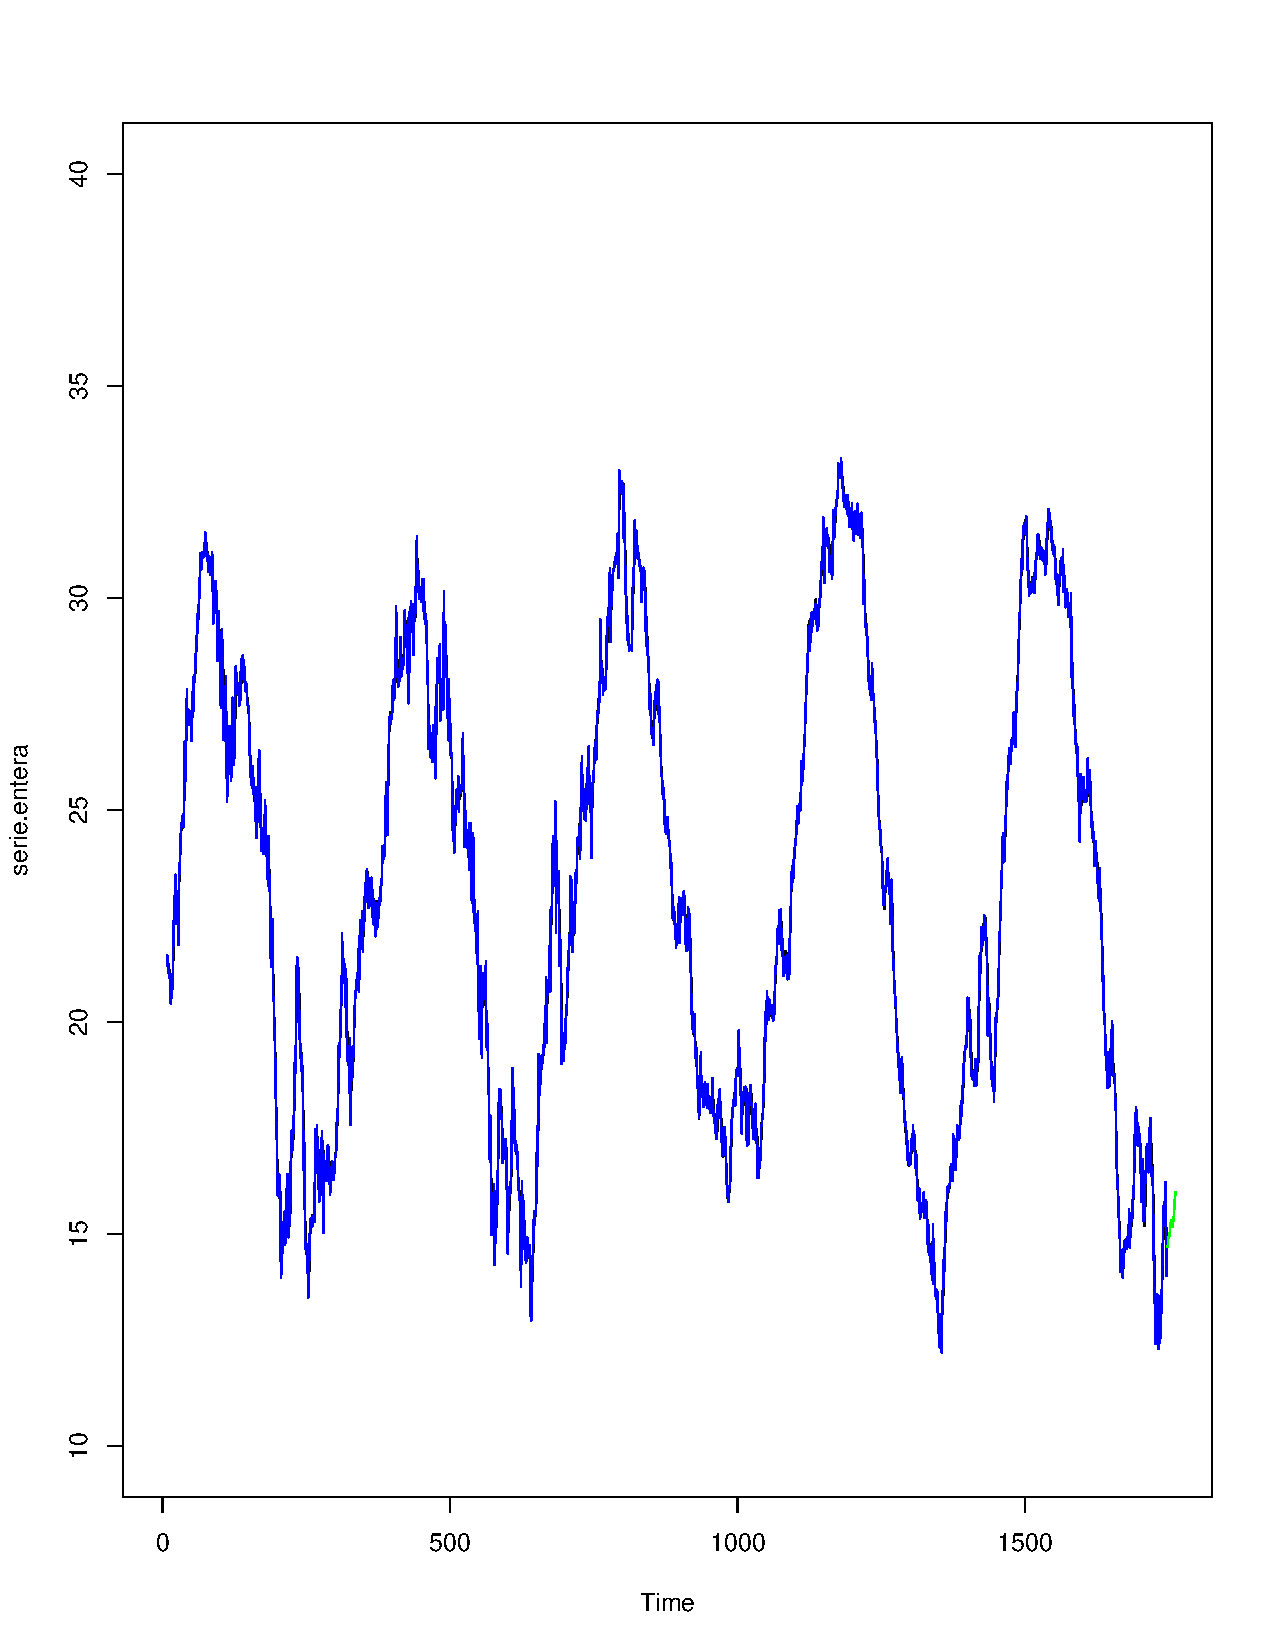
\includegraphics[width=100mm]{imagenes/pred_ar1.pdf}
	\caption{Predicción temperatura máxima para la primera semana de marzo}
	\label{fig:15}
\end{figure}

En la esquina derecha de la imagen, se puede ver en verde la predicción del modelo; la cual parece acertada, ya que normalmente a partir de marzo las temperaturas empiezan a incrementar.
 
\section{Predicción mensual}
Para la predicción mensual se seguirá los mismos pasos que para el estudio de la serie con datos diarios. Para obtener la temperatura media por mes, se utilizará la función \textit{group\_by}, \textit{summarise} y pipelines de la librería \textit{dplyr}, antes se leeran los datos y se imputarán. La serie resultante es la siguiente. Una vez se va a crear la serie, se debe especificar la frecuencia como 12, ya que estamos tratando con meses.

\begin{figure}[H]
	\centering
	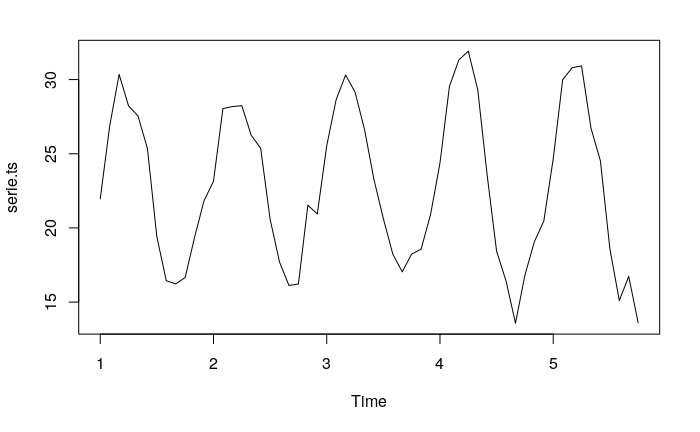
\includegraphics[width=100mm]{imagenes/serie_mean.png}
	\caption{Serie temperatura media}
	\label{fig:16}
\end{figure}

La descomposición de la serie es la siguiente.

\begin{figure}[H]
	\centering
	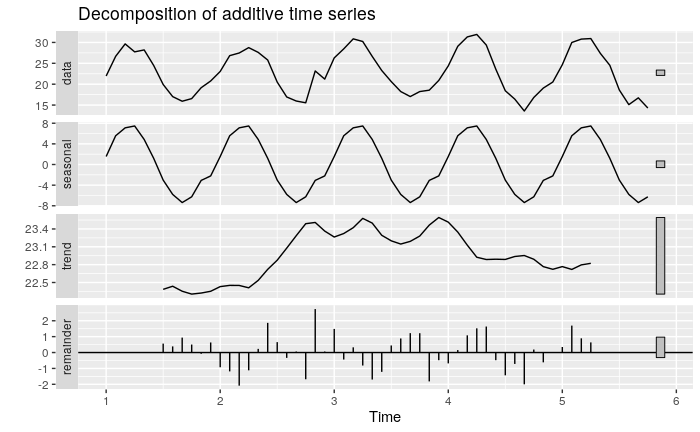
\includegraphics[width=100mm]{imagenes/decompose_mean.png}
	\caption{Descomposición serie media}
	\label{fig:17}
\end{figure}

Al igual que antes, no hay una componente estacional, y sí que hay una componente estacional, la cual tendremos que eliminar para poder comprobar si la serie es estacionaria. Antes de eliminar la estacionalidad, se va a separar la serie en train y test; para train se utilizarán 4 años y el resto para test. La separación en train y test es la que se muestra a continuación.

\begin{figure}[H]
	\centering
	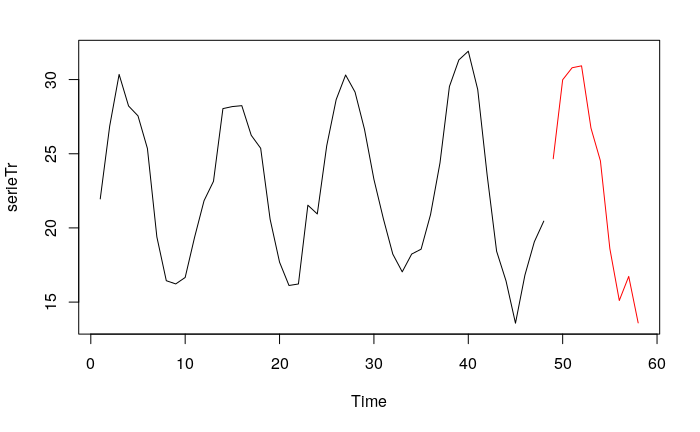
\includegraphics[width=100mm]{imagenes/train_test_mean.png}
	\caption{Conjuntos de test y train}
	\label{fig:18}
\end{figure}

Para eliminar la estacionalidad, se debe hacer lo mismo que en el ejercicio anterior; obtener la componente estacional y restar a cada conjunto dicha componente. La serie sin estacionalidad sería la siguiente.

\begin{figure}[H]
	\centering
	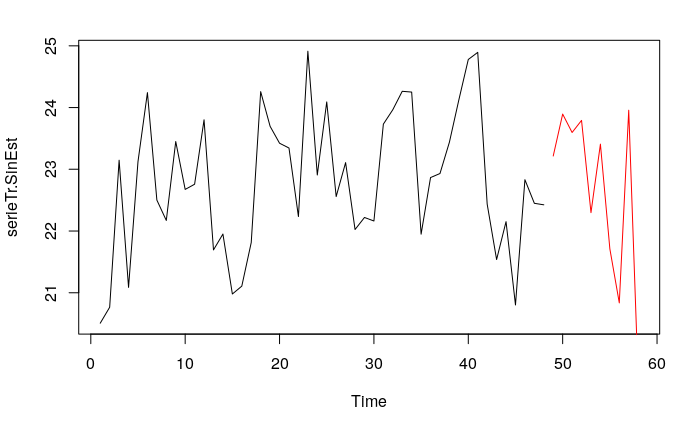
\includegraphics[width=100mm]{imagenes/sin_est_mean.png}
	\caption{Serie sin estacionalidad}
	\label{fig:19}
\end{figure}


Ahora comprobaremos si la serie es estacionaria, para ello se utilizará el test de \textit{Dickey-Fuller} y la gráfica \textit{ACF}. Si pasa el test y la gráfica desciende rápidamente a 0 sabemos que la serie es estacionaria.

\begin{figure}[H]
	\centering
	\subfigure[Test estacionaria]{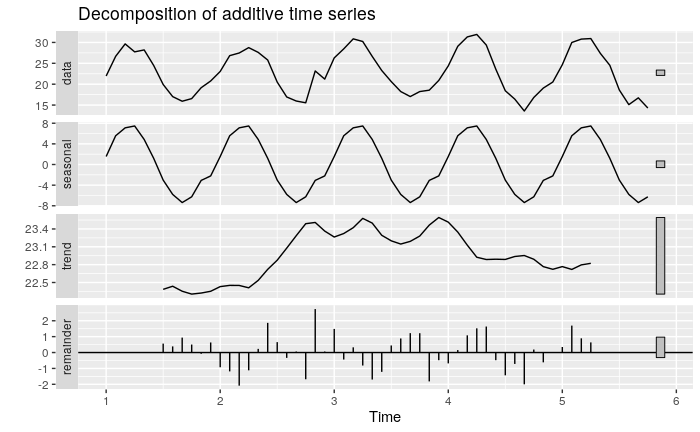
\includegraphics[width=60mm]{imagenes/decompose_mean.png}}
	\subfigure[Gráfica ACF]{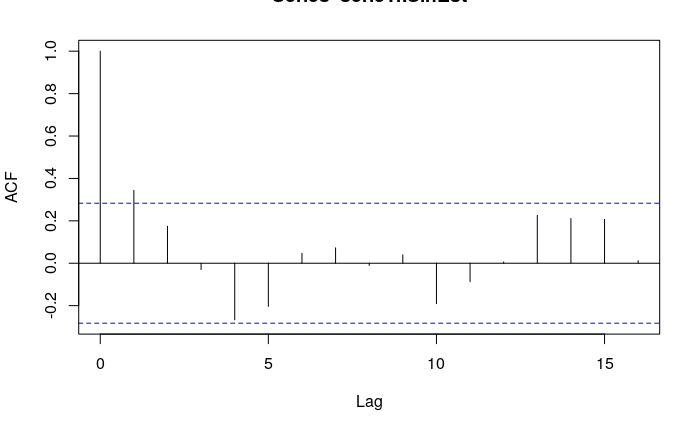
\includegraphics[width=60mm]{imagenes/acf_mean.png}}
	\caption{Estacionariedad y ACF serie}
	\label{fig:20}
\end{figure}

Como se puede ver, pasa el test y la gráfica desciende rápidamente a 0, por lo que es estacionaria. Lo siguiente será decidir que modelo utilizar, para ello se utilizará tanto la gráfica \textit{ACF} como la gráfica \textit{PACF}.

\begin{figure}[H]
	\centering
	\subfigure[Gráfica ACF]{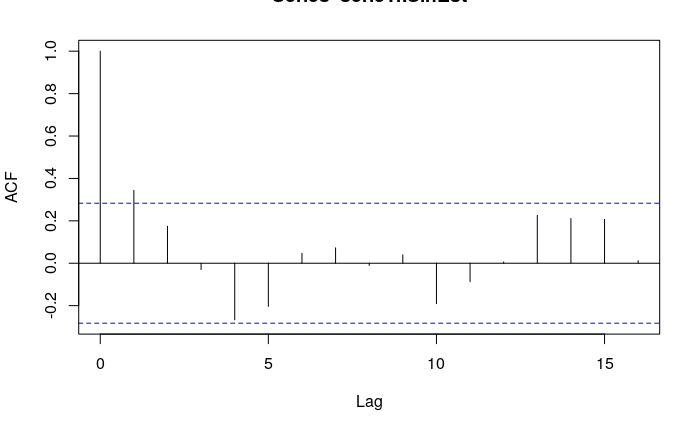
\includegraphics[width=60mm]{imagenes/acf_mean.png}}
	\subfigure[Gráfica PACF]{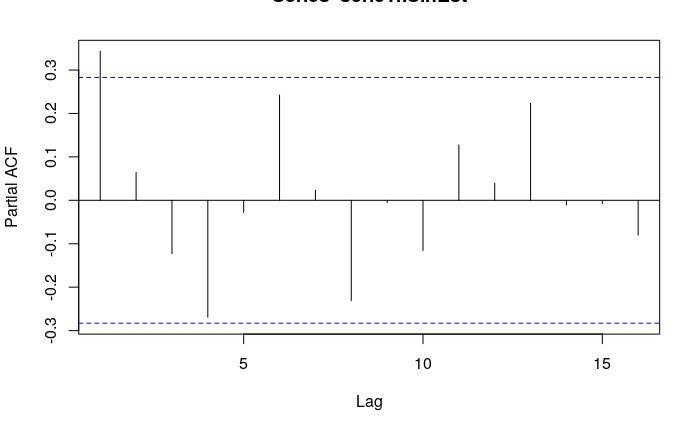
\includegraphics[width=60mm]{imagenes/pacf_mean.png}}
	\caption{Gráficas ACF y PACF serie medias}
	\label{fig:21}
\end{figure}

Por lo que se puede ver en las gráfica, parece que claramente se debe utilizar un modelo MA(2). Para crear el modelo se utilizará \textit{ARIMA}, tras esto, se comprobará el ajuste del modelo con los datos de train y test y con los test de \textit{Shapiro}, \textit{Jarque-Bera} y \textit{Box-Pierce}.

\begin{figure}[H]
	\centering
	\subfigure[Test MA2]{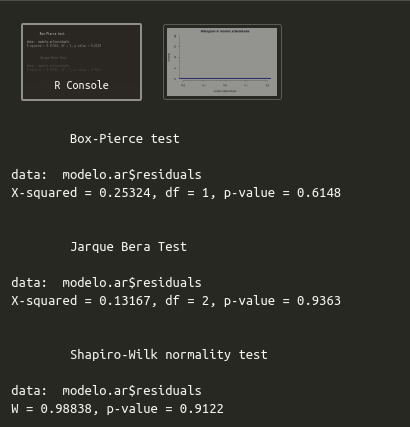
\includegraphics[width=60mm]{imagenes/test_mean_ma2.png}}
	\subfigure[Ajuste MA2]{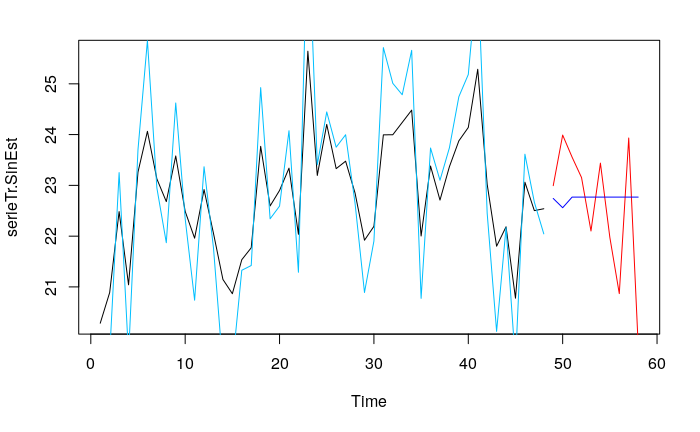
\includegraphics[width=60mm]{imagenes/ajuste_mean.png}}
	\subfigure[Ajuste MA2 con estacionalidad]{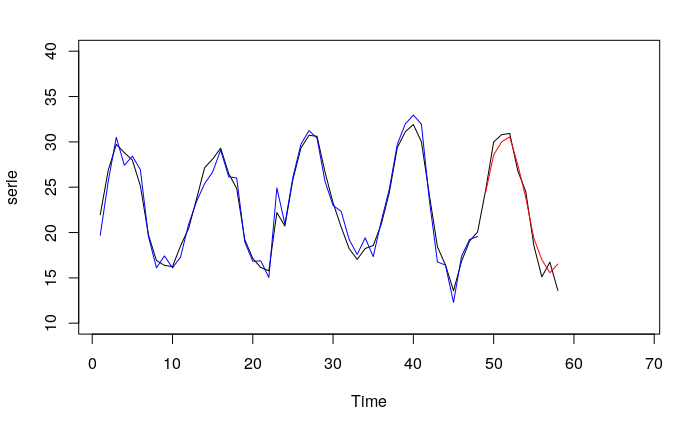
\includegraphics[width=60mm]{imagenes/ajuste_mean_serie.png}}
	\caption{Resultados modelo MA2}
	\label{fig:22}
\end{figure}

Por lo que se puede ver, el ajuste parece bueno. Aunque no pase los test de normalidad, sí que pasa el test de \textit{Box-Pierce}. Posiblemente no pase los test de normalidad porque tenemos bastantes pocos datos para train y este tipo de test suelen necesitar bastantes datos para ser fiables. Por ello, utilizaremos este modelo para realizar la predicción de los dos siguientes meses. Al igual que en el ejercicio anterior, ahora se utilizará la serie entera, se eliminará la estacionalidad y se obtendrá un modelo MA(2) entrenados con esos datos, una vez obtenidos las predicciones se volverá a añadir la estacionalidad y se comentarán los resultados.

\begin{figure}[H]
	\centering
	\includegraphics[width=100mm]{imagenes/pred_mean.pdf}
	\caption{Predicción serie temperatura media}
	\label{fig:23}
\end{figure}

Los resultados obtenidos en la predicción tienen bastante sentido, ya que es normal que la temperatura media en estos meses continúe aumentando, además si nos fijamos en meses iguales de otros años, los valores son muy parecidos a los obtenidos por la predicción; por lo que podemos concluir que el modelo obtenido consigue un buen ajuste para predecir la temperatura.
